
\chapter{绪论}
\label{chap:introduction}
\section{研究背景与意义}
	自互联网诞生以来,用户寻找信息的方法经历了几个阶段。早期的用户主要靠直接记住感兴趣网站的网址来寻找内容,直接促使Yahoo!提出了分类目录系统,将网站分门别类方便用户查询。但随着信息越来越多,分类目录也只能记录少量的网站,于是产生了搜索引擎。以Google为代表的搜索引擎可以让用户通过关键词找到自己需要的信息,但是,搜索引擎需要用户主动的提供显式关键词来寻找信息,因此它不能解决用户的更多的潜在需求,当用户无法精准描述自己的需求时,搜索引擎就无能为力了,于是又催生出推荐系统\citep{recmd-system}。以亚马逊电商官网为代表的推荐系统是一种帮助用户快速发现有用信息的工具,和搜索引擎不同的是推荐系统不需要提供明确的需求,而是通过分析用户的历史行为来给用户画像建模\citep{demo-data}从而主动给用户推荐出能够满足他们兴趣和需求的信息。因此,从某种意义上说推荐系统和搜索引擎是两个互补的工具。搜索引擎满足用户显式的需求,而推荐系统能够在用户没有明确目的的时候帮助他们发现潜在的需要。随着物联网和用户终端设备的发展,人们逐渐从信息的匮乏时代走进了信息的过载时代。无论是作为信息消费者的普通用户,还是作为信息生产者的提供商面临着数据爆炸时代的挑战。作为用户,如何从充斥着大量噪声的大数据中找到自己感兴趣的信息是一件非常耗时费力的事情,笔者曾有过这样的一种购物体验:在淘宝商城购买一台笔记本电脑,花费了一上午的时间才浏览、比较完所有的 thinkpad 品牌商家店面,如\autoref{fig:hl_taobao}。
	\begin{figure}
		\centering
		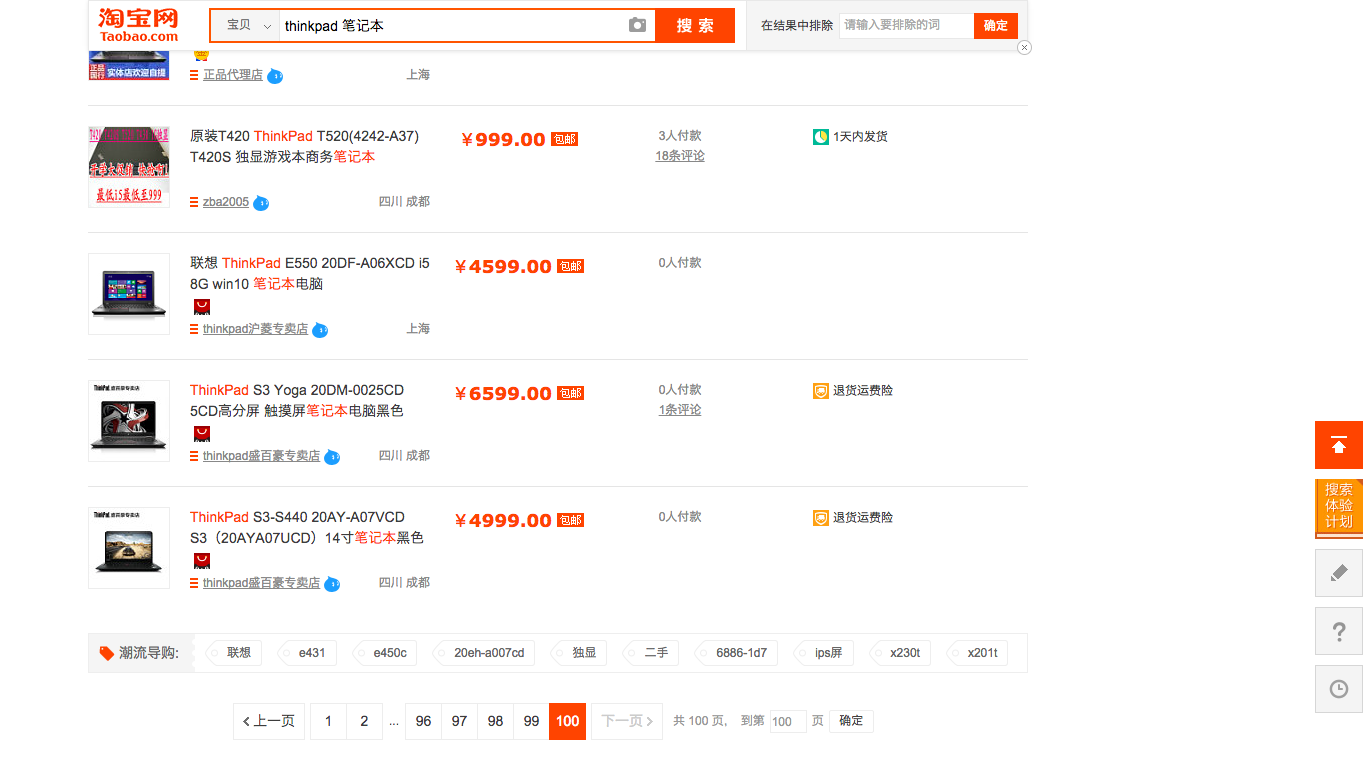
\includegraphics[width=0.9\textwidth]{hl_taobao}
		\figcaption{淘宝购物搜索图}
		\label{fig:hl_taobao}
	\end{figure}
	而作为互联网企业,如何让自己生产的信息不埋没在大数据洪流中而受到潜在用户的充分关注,这也是其所要解决的一个课题,很多企业已经或者正在开发适合本公司的推荐系统来解决这一矛盾。传统的推荐系统通过分析用户的数据,通过对商品打分、排序找到用户感兴趣的商品,然后推荐给他们,但是传统的推荐系统在大数据时代也面临着严峻的问题,典型的问题有数据稀疏问题、新用户问题、马太效应、实时推荐问题和用户兴趣变动问题。

	基于这种现实,人们开始回归问题的本质即以人为本,用数据说话,通过分析、收集所有与用户有关的数据,为每个用户建立、维护一个独一无二的用户画像,用户画像的最大优点在于它能主动收集用户的基本人口数据、长期兴趣和短期兴趣,而且此信息是动态更新的,也就是说随着时间的推移,用户的兴趣在逐渐改变,用户画像里的兴趣标签也会随之改变。因此,用户画像大大的提高了互联网企业的用户体验。用户画像的主要任务就是让推荐系统更了解用户,一方面让信息更加针对性的展现在只对它有兴趣的用户面前,提升商品的转化率,另一方面协助用户发现自己潜在感兴趣的信息,提升用户的满意度,于是实现了消费者和生产者的双赢。

\section{推荐系统的简介}
推荐系统的研究和很多早期的研究相关,比如认知科学\citep{cognitive-science},信息检索和预测理论\citep{Forecast-principle}。随着互联网的兴起,研究人员开始研究如何利用用户对物品行为数据来预测用户的兴趣并给用户做推荐\citep{cf-sn}。推荐系统开始成为一个比较独立的研究问题。到2006年为止推荐系统的研究主要集中在基于邻域的协同过滤算法,目前工业界应用最广泛、最知名的算法应该就是亚马逊开发并使用的协同过滤算法\citep{Amazon-cf}。推荐系统推荐给用户的商品首先不能与用户购买过的商品重复,其次也不能与用户刚浏览过的商品太相关。推荐系统的形式化定义如:设C是所有用户的集合,S是所有可以推荐给用户的主题的集合。实际上,C和S集合的规模通常很大,如上百万的顾客以及上万款手机主题。设函数u()可以计算主题s对用户c的推荐度R,即$u=C\times S \rightarrow R$,R是一定范围内的全序的非负实数,推荐要研究的问题就是找到推荐度R最大的那些主题S*,如\autoref{equ:fromal}。
\begin{equation}
\forall c \in C,S^{*}=arg  max_{s \in S} u(c,s)
\label{equ:fromal}
\end{equation}

	\subsection{推荐系统的产生与发展}
	随着科学技术与信息传播的迅猛发展,人类社会进入了一个全新的大数据时代,互联网和物联网无处不在的影响着人类生活的方方面面,并颠覆性改变了人们的生活方式,互联网用户既代表了网络信息的消费者,也代表了网络内容的生产者。尤其是随着Web 2.0时代的到来,社交化网络媒体的异军突起,互联网中的信息量呈指数级增长,而由于用户的辨别能力有限,使得其在庞大且复杂的互联网信息中找寻有用信息的成本巨大,这就是所谓的信息过载问题\citep{info-overload, info-overload:1}。搜索引擎和推荐系统的出现为用户解决信息过载提供了非常重要的技术手段。搜索引擎是被动的,用户在搜索互联网中的信息时需要在搜索引擎中输入关键词,搜索引擎根据输入在系统后台进行信息匹配,将与用户查询相关的信息展示给用户。但是当用户无法精确描述自己需求时,搜索引擎就无能为力了。推荐系统是主动的,用户不需要提供明确的需求,而是通过分析用户的历史行为来对用户进行分析,从而主动给用户推荐可能满足他们兴趣和需求的信息。因此搜索引擎和推荐系统是两个互补的技术手段。

	推荐系统概念是1995年在美国人工智能协会\citep{recmd-history}上由CMU大学的教授Robert Armstrong首先提出并推出了推荐系统的原型系统——Web Watcher。随后推荐系统的研究工作开始慢慢壮大。第一个正式商用的推荐系统是1996年Yahoo网站推出的个性化入口MyYahoo。21新世纪推荐系统的研究与应用随着电子商务的快速发展而风起云涌,各大电子商务网站都开发、部署了推荐系统,Amazon公司称其网站中35\%的营业额来自于自身的推荐系统。2006年美国的DVD租赁公司Netflix\citep{recmd-netflix}在网上公开设立了一个推荐算法竞赛并公开了真实网站中的一部分数据,包含用户对电影的评分。Netflix竞赛有效地推动了学术界和产业界对推荐算法的兴趣,很多有效的算法在此阶段被提了出来。

	近几年随着电子商务蓬勃发展,推荐系统在互联网中的优势地位也越来越明显。在国外比较著名的电子商务网站有Amazon和eBay,其中Amazon平台中采用的推荐算法是非常成功的。在国内比较典型的电子商务平台网站有淘宝网、网页云音乐、爱奇艺PPS等。在这些电子商务平台中,网站提供的商品数量不计其数,网站中的用户规模也非常巨大。据不完全统计天猫商城中的商品数量已经超过了5000万。在商品数量如此庞大的电商网站中,如果用户仅仅根据自己的购买意图输入关键字查询只会得到很多用户很难区分的相似结果,也不便用户做出选择。因此推荐系统作为能够根据用户兴趣\citep{user-interest}为用户推荐商品的主要途径,从而为用户在购物的选择中提供建议的需求非常明显。目前比较成功的电子商务网站中,都不同程度地利用推荐系统在用户购物的同时为用户推荐一些商品,从而提高商品的销售额。另一方面,随着以智能手机为代表的物联网推动了移动互联网的发展。在用户在连入移动互联网的过程中,其所处的地理位置信息可以非常准确地被获取,并由此出现了大量的基于用户位置信息的网站。国外比较著名的有Uber和Coupons。国内著名的有滴滴出行和美团网。例如,在美团网这种基于位置服务的网站中,用户可以根据自己的当前位置搜索餐馆、酒店、影院、旅游景点等信息服务。同时,可以对当前位置下的各类信息进行点评,为自己在现实世界中的体验打分,分享自己的经验与感受。当用户使用这类基于位置的网站服务时,同样会遭遇信息过载问题。推荐系统可以根据用户的位置信息为用户推荐当前位置下用户感兴趣的内容,为用户提供符合其真正需要的内容,提升用户对网站的满意度。

	随着社交网络的深入人心,用户在互联网中的行为不再局限于获取信息,更多的是与网络上的其他用户进行互动。国外著名的社交网络有Facebook、Twitter等,国内的社交网络有微信、米聊等。在社交网站中用户不再是单个的个体,而是与网络中的很多人具有了错综复杂的社交关系链。社交网络中最重要的资源就是用户与用户之间的这种联系。社交网络中用户间的关系是多维度的,建立社交关系的因素可能是在现实世界中是亲人、同学、同事、朋友关系,也可能只是网络中的虚拟朋友,比如都是有着共同爱好的会员成员。在社交网络中用户与用户之间的联系紧密度反映了用户之间的信任关系,用户不在是一个个体存在,其在社交网络中的行为或多或少地会受到其他用户关系的影响。因此推荐系统在这类社交网站中的研究与应用应该考虑用户社交的影响。

	现如今推荐系统在很多领域得到了广泛的应用,如出租车推荐、商品推荐、美餐推荐、电影推荐和音乐推荐,几乎囊括了人类的吃住行穿四大领域,团购网站美团网早已经利用推荐系统提供面向不同业务的个性化服务:1,猜你喜欢:美团最重要的推荐产品,目标是让用户打开美团App的时候,可以最快找到用户想要的团购服务;2,首页频道推荐:若干频道是固定的,若干频道是根据用户的个人偏好推荐出来的;3,今日推荐个性化推送:美团的个性化推送的产品,目的是在用户打开美团App前,就把用户最感兴趣的服务推送给用户,促使用户点击及下单,从而提高用户的活跃度;4,品类列表的个性化排序:美团首页的那些品类频道区。

	自推荐系统诞生后学术界对其关注的兴趣度也越来越大。从1999年开始美国计算机学会每年召开电子商务研讨会以来,发表的与推荐系统相关的论文数以千计。ACM信息检索专业组在2001年开始把推荐系统作为该会议的一个独立研究主题。同年召开的人工智能联合大会也将推荐系统作为一个单独的主题。目前为止数据库、数据挖掘、人工智能、机器学习方面的重要国际会议(如KDD、AAAI、ICML等)都有大量与推荐系统相关的研究成果发表。同时第一个以推荐系统命名的国际会议ACM Recommender Systems Conference 于2007年首次举办。在近几年的数据挖掘及知识发现国际会议举办的竞赛中,连续两年的竞赛主题都是推荐系统。2011年的KDD CUP 竞赛中,两个竞赛题目分别为音乐评分预测和识别音乐是否被用户评分(\href{http://www.kdd.org/kdd2011/kddcup.shtml}{www.kddcup2011.org})。2012年的KDD CUP 竞赛中,两个竞赛题目分别为腾讯微博中的好友推荐和计算广告中的点击率预测。(\href{www.kddcup2012.org}{www.kddcup2012.org})

	\subsection{推荐系统的应用}
	推荐系统改变了没有活力的网站与其用户通信的方式。无需提供一种静态体验,让用户搜索并可能购买产品,推荐系统加强了交互,以提供内容更丰富的体验。推荐系统根据用户过去的购买和搜索历史,以及其他用户的行为,自主地为各个用户识别推荐内容。个性化推荐的最大的优点在于它能收集用户特征资料并根据用户特征,如兴趣偏好,为用户主动作出个性化的推荐。而且,系统给出的推荐是可以实时更新的,即当系统中的商品库或用户特征库发生改变时,给出的推荐序列会自动改变。这就大大提高了电子商务活动的简便性和有效性,同时也提高了企业的服务水平。总体说来,一个成功的个性化推荐系统的作用主要表现在以下几个方面:
	\begin{enumerate}[(1)]
	\item 将电子商务网站的浏览者转变为购买者:电子商务系统的访问者在浏览过程中经常并没有购买欲望,个性化推荐系统能够向用户推荐他们感兴趣的商品,从而促成购买过程。
	\item 提高电子商务网站的交叉销售能力:个性化推荐系统在用户购买过程中向用户提供其他有价值的商品推荐,用户能够从系统提供的推荐列表中购买自己确实需要但在购买过程中没有想到的商品,从而有效提高电子商务系统的交叉销售。
	\item 提高客户对电子商务网站的忠诚度:与传统的商务模式相比,电子商务系统使得用户拥有越来越多的选择,用户更换商家极其方便,只需要点击一两次鼠标就可以在不同的电子商务系统之间跳转。个性化推荐系统分析用户的购买习惯,根据用户需求向用户提供有价值的商品推荐。如果推荐系统的推荐质量很高,那么用户会对该推荐系统产生依赖。因此,个性化推荐系统不仅能够为用户提供个性化的推荐服务,而且能与用户建立长期稳定的关系,从而有效保留客户,提高客户的忠诚度,防止客户流失。
	\end{enumerate}

\section{用户画像的简介}
	用户,指企业的目标用户,或者是构成现有用户的大部分群体的统称。画像,是对一个事物的客观的、准确的、可视化的描述。用户画像就是能够客观、准确、可视化地描述目标用户的模型或方法。为用户画像的焦点工作就是为用户打标签,而一个标签通常是人为规定的高度精炼的特征标识,如年龄、性别、地域、用户偏好等,最后将用户的所有标签综合来看,基本就可以勾勒出该用户的立体画像了。
	\subsection{用户画像的产生背景}
	在互联网逐渐步入大数据时代后,不可避免的给企业及消费者行为带来一系列改变与重塑。其中最大的变化莫过于,消费者的一切行为在企业面前似乎都将是可视化的。随着大数据技术的深入研究与应用,企业的专注点开始回归本质,日益聚焦于怎样利用大数据来为精准刻画用户,进而深入挖掘潜在的商业价值。于是,用户画像的概念也就应运而生。大数据时代的用户画像代表了一个用户的信息全貌,为进一步精准、快速地分析用户行为习惯、消费习惯等重要信息,提供了足够的数据基础。用户画像即用户信息标签化,就是企业通过收集与分析消费者社会属性、生活习惯、消费行为等主要信息的数据之后,抽象出一个用户的商业全貌是企业应用大数据技术的基本方式。用户画像为企业提供了足够的信息基础,能够帮助企业快速找到精准用户群体以及用户需求等更为广泛的反馈信息。2015上半年,我国网民已达到6.68亿,预计年底能够顺利突破7亿,其中使用手机上网人群占整体88.9\%。不同于传统PC上网,每个家庭共用一台设备,手机上网存在着独特性、唯一性和私密性的特点,每个人的手机都是一套独特的生态系统。因此,将有相同特征的用户抽象成一个代表,可以极大方便开发者研究用户构成和分布,精准定义用户。中国在各方面都是很大的长尾市场,互联网很大程度上弥补了信息的不对称,移动互联网又让把信息在精准送达到任意一个用户面前,面临在所有互联网企业面前的问题是,如何才能将流量变现,实现产品的商业价值呢?为了充分发挥大数据的真正价值,第一步理应是整理数据。而整理数据的阶段目的是完成目标用户或者是现有用户的画像,只有得到了准确的用户画像,才能更好的达到流量变现的目的。
	\subsection{用户画像的应用}
	用户画像的意义在于完善产品运营提升用户体验,提升盈利,根据产品特点,找到目标用户,在用户偏好的渠道上与其交互,促成购买,实现精准运营和营销。于此同时,用户画像改变了以往闭门造车式的商业交易模式,通过事先调研用户需求反馈,设计制造出更适合用户的产品。
	\begin{itemize}
	\item 完善及扩充用户信息:用户画像的首要动机就是了解用户,这样才能够提供更优质的服务。但是在实际中用户的信息提供得不尽完整,如对于没有填写性别信息的用户,用户画像通过分析用户语音数据识别其性别,尽可能多的为推荐系统提供正确的基础特征。
	\item 打造健康的生态圈:在掌握用户信息的基础上,平台就可以对自身的状况进行分析,从相对宏观的基础上把握主题市场的生态环境,挖掘设计作品的最大价值,帮助设计师提高收入。例如通过对用户信息的聚类,能够对用户进行人群的划分,掌握不同人群的活跃程度、行为及兴趣偏好,热门商品的传播方式和流行引爆点等。
	\item 支撑推荐系统的精准推荐:精准推荐的前提是对用户的清晰认知。在实际场景中,影响用户对商品的使用黏度的因素很多,在这种情况下,利用用户画像可以对用户的“贴身跟踪”就能及时发现薄弱环节,因此从用户打开应用网上商店到退出使用,其间的每一步情况都被快的记录在案:哪一天退出的,哪一步退出的,退出之后“跳转”到什么软件等等。据此,用户画像也实现了用户另外一个纬度的归类,分清哪部分是忠实用户,哪部分可能是潜在的忠实用户,哪些则是已经流失的;更进一步来看流失的原因:因为代金券没有了流失?主题包质量不好流失?这些都是下一步精准推荐的依据,无论是基于兴趣的推荐提升用户价值,精准的广告投放提升商业价值,还是针对特定用户群体的内容运营,用户画像都是其必不可少的基础支撑。直接地,用户画像可以用于兴趣匹配、关系匹配的推荐和投放;间接地,可以基于用户画像中相似的兴趣、关系及行为模式去推动用户兴趣和设计师的无缝对接。
	\item 市场安全领域的应用:随着电子商务的发展,商家会通过各种活动形式的补贴来获取用户、培养用户的消费习惯,但同时也催生一些通过刷排行榜、刷红包的用户,这些行为距离欺诈只有一步之遥,但他们的存在严重破环了市场的稳定,侵占了活动的资源。其中一个有效的解决方案就是利用用户画像沉淀方法设置促销活动门槛,即通过记录用户的注册时间、历史登陆次数、常用IP地址等,最大程度上隔离掉僵尸账号,保证市场的稳定发展。
	\end{itemize}

\section{工程背景}
	小米科技作为国内发展较快的互联网企业,活跃用户过亿,移动端用户比例高,有着大量的用户和丰富的用户行为,这些为推荐系统的应用和优化提供了不可或缺的条件,我们基于MIUI主题应用开发的手机主题推荐系统,作为用户和主题包之间的桥梁,体现出超强的变现能力。但现有的手机主题推荐系统也面临着一些问题。
	\begin{enumerate}[(1)]
	\item 新用户冷启动问题。我们当前使用的推荐算法,包括最近邻的协同过滤算法、PageRank排序算法、关联规则挖掘是根据给定用户对某些物品的行为数据,给每个用户推荐Top-N个其最喜欢的物品,当一个新用户进入一个站点时,我们对他的兴趣爱好还一无所知,这时如何做出推荐是一个很重要的问题。现有的机制是向用户推荐那写普遍反映比较好的物品,也就是说,推荐完全是基于物品的,这就会使热门的商品越来越热,冷门的商品越来越冷,但是代价就是加剧商品的马太效应。

	\item 数据稀疏问题,通过观察我们发现只有约10\%的用户有过多于10款主题行为记录,意味着大多数主题包处于待挖掘状态,然后,这又是一个蛋和鸡的问题:要形成好的推荐,首先需要有大量的用户行为支持,这样才能得到足够多的推荐数据,这里问题的关键在于推荐系统如何首先能在数据稀疏的情况下给出优质的服务,打破这个闭环。

	\item 不断变化的用户喜好,这个问题主要分为俩类:1、用户一直喜欢某种类型的主题包,只是长时间没有机会接触,如一位男性用户喜欢少女主题包款式,虽然不会主动查找,但如果不经意看到一款制作精美的美女主题包,可能还是会购买,这就是用户的长期兴趣。2、用户之前喜欢某种类型的主题包,之后转为喜欢另外一类主题包,如用户刚开始喜欢清纯系,后来转为温柔系,这时如果向用户推荐温柔系美女主题包更有可能被其接受,这就是用户的短期兴趣。

	\item 重复推荐的问题,手机主题包属于电子虚拟商品,它的特性是第一次下载需要购买,之后下载则免费,现有的推荐系统会重复推荐用户之前购买过的主题,导致占用有限的推荐位来显示无法变现的信息,不经济,并且会给用户一种不专业、不智能的体验。

	\item 其他问题,如推荐商品长尾性有待加强、隐性喜好难以挖掘、偏激的用户和另类的产品、推荐系统的作弊行为、用户请求量大等。这些问题相对来讲影响范围小,本论文不做过多讨论。
	\end{enumerate}

	我们发现,如果在数据层和推荐系统之间加一个用户画像模块,会有效提升推荐系统的各项性能。1、对于新用户冷启动问题、数据稀疏问题,关键是收集足够多的用户基本信息,在没有或者只有少量用户行为的情况下依靠用户画像对用户推荐比较合理的主题。2、对于不断变化的用户喜好,我们通过用户画像存储用户用户长期,通过用户兴趣探索获得用户短期兴趣,并针对手机主题市场的特点,利用线性衰减算法融合用户画像和用户兴趣探索,使得推荐结果能兼顾俩者。3、对于重复推荐的问题,我们在用户画像中维护一个白名单,用来存储用户曾购买过的所有主题信息,格式为(itemId,buyTime)这样的二元组。除此之外,我们也通过探索用户小众兴趣提升推荐系统的长尾发掘能力,加强了对小众主题包的推荐力度。主要思路是分析用户所有的行为数据,针对冷门主题(冷门主题包含的标签一般是小众标签)的行为会赋予一个倾斜因子,这样会使得兴趣探索标签候选集中的小众标签占大多数,而如果用户对这些主题的满意度也很高,则说明这是一个成功的兴趣探索。

	总之,我们采用构建用户画像的办法分析、处理、挖掘现有的用户信息,尽可能多的识别用户基础特征和兴趣偏好,达到优化推荐系统的目的,后续需求包括广告投放、定向营销、流量变现等也都围绕建立更细致、准确的人群画像展开。
\section{推荐系统开源项目介绍}
工欲善其事,必先利器,关于大数据,有很多令人兴奋的事情,但如何分析、利用它也带来了很多困惑。好在开源观念盛行的今天,有一些在大数据领域领先的免费开源技术可供利用。
\begin{itemize}
	\item Apache Hadoop:Hadoop是一个由Apache基金会所开发的分布式系统基础架构,是一种用于分布式存储和处理商用硬件上大型数据集的开源框架,可让各企业迅速从海量结构化和非结构化数据中获得洞察力。Hadoop的框架最核心的设计就是HDFS和MapReduce。HDFS为海量的数据提供了存储,则MapReduce为海量的数据提供了计算。HDFS有高容错性的特点,并且设计用来部署在低廉的硬件上;而且它提供高吞吐量来访问应用程序的数据,适合那些有着超大数据的应用程序。MapReduce 本身就是用于并行处理大数据集的软件框架,其根源是函数性编程中的 map 和 reduce 函数。它由两个可能包含有许多实例的操作组成。Map 函数接受一组数据并将其转换为一个键/值对列表,输入域中的每个元素对应一个键/值对。
	\item Apache Hive:Hive是建立在 Hadoop 上的数据仓库基础构架。它提供了一系列的工具,可以用来进行数据提取转化加载,这是一种可以存储、查询和分析存储在Hadoop中的大规模数据的机制。Hive定义了简单的类SQL查询语言,称为HQL,它允许熟悉SQL的用户查询数据。同时,这个语言也允许熟悉 MapReduce 开发者的开发自定义的 mapper 和 reducer 来处理内建的 mapper 和 reducer 无法完成的复杂的分析工作,十分适合数据仓库的统计分析。
	\item Apache Spark:Spark是加州大学伯克利分校所开源的类Hadoop的通用并行框架,Spark拥有 Hadoop 所具有的优点;但不同于 Hadoop 的是Job中间输出结果可以保存在内存中,从而不再需要读写HDFS,因此Spark能更好地适用于数据挖掘与机器学习等需要迭代的MapReduce的算法。
	\item Apache Kafka:Kafka 是一种高吞吐量的分布式发布订阅消息系统,它可以处理消费者规模的网站中的所有用户行为流数据。这种用户行为流数据是在现代网络上的许多社会功能的一个关键因素。这些数据通常是由于吞吐量的要求而通过处理日志和日志聚合来解决。对于像Hadoop的一样的日志数据和离线分析系统,但又要求实时处理的限制,Kafka一个可行的解决方案。其目的是通过Hadoop的并行加载机制来统一线上和离线的消息处理,也是为了通过集群机来提供实时的消费。
\end{itemize}

\section{论文结构}
	本文的其余正文内容由以下章节组成:
	\begin{itemize}
		\item 第二章首先介绍了推荐系统基本概念和排序模型,包括数据挖掘算法\citep{date-mining}和信息提取技术\citep{info-retrieval}的应用,然后详细介绍了用户画像和用户兴趣探索。
		\item 第三章主要讨论了如何利用用户画像建模解决推荐系统的冷启动问题,从而改善推荐系统的新用户留存率。最后给出了相关的实验结果及分析。
		\item 第四章主要讨论了如何利用用户兴趣探索跟踪用户动态并挖掘用户小众兴趣,从而提升推荐系统的长尾效应\citep{long-tail},文中给出了相关的实验结果及分析。
		\item 第五章是论文的结束语和展望,在对目前工作简要总结的基础上,提出了推荐系统下一步研究的任务和方向。
	\end{itemize}